\documentclass{article}

\usepackage{inputenc}[utf8]
\usepackage[T1]{fontenc}
\usepackage[a4paper]{geometry}
\usepackage{fancyhdr}
\usepackage{url}
\usepackage{hyperref}
\usepackage[ngerman]{babel}
\usepackage{graphicx}
\usepackage{pgfplots}
\usepackage{amsmath}
\usepackage{amssymb}
\usepackage{amsthm}
\usepackage{nicefrac}

\usepackage{pdflscape}
\usepackage{caption}
\usepackage{subcaption}

% Generate external pdf and import
\pgfplotsset{width=9cm,compat=1.9}

\title{{\Huge Aufgabenblatt 05}\\Einführung in die Kryptographie PS}
\author{Andreas Schlager}


\begin{document}
    \pagestyle{fancy}
    \fancyhead{}
    \fancyhead[L]{Aufgabenblatt 05}
    \fancyhead[R]{Einführung in die Kryptographie}
    \fancyfoot{}
    \fancyfoot[L]{Andreas Schlager}
    \fancyfoot[R]{\thepage}
    \maketitle
    \tableofcontents
    \newpage

    \section{Aufgabe 17}
\textit{Fortsetzung Aufgabe 16.): Bestimmen Sie mit der in der VO besprochenen Methode
mit Iteration über die Länge der Keys unter Berechnung der Hamming Distanz (Slide
65, 2. Verfahren) die Länge des Keys in dem in Aufgabe 16.) realisierten short Key
XOR Verschlüsselungsverfahren.}\vspace*{1em}\newline
Wie bereits in der vorherigen Aufgabe beschrieben, wird ein Plaintext durch ein Short-Key-XOR-Verfahren verschlüsselt. Der verwendete Schlüssel sowie seine Länge sind dabei unbekannt. Gegeben ist lediglich der resultierende Ciphertext.
Zur Bestimmung der Schlüssellänge wird die durchschnittliche Hamming-Distanz benachbarter Blöcke des Ciphertexts analysiert. Hierfür werden unterschiedliche Blockgrößen getestet, wobei die jeweilige Blockgröße der vermuteten Schlüssellänge entspricht.
Die Funktion \verb|average_hamming_distance| berechnet die durchschnittliche Hamming-Distanz zweier aufeinanderfolgender Blöcke für einen gegebenen Ciphertext:
\begin{verbatim}
fn average_hamming_distance(cipher: &[u8], block_size: usize) -> f32 {
    let cipher_blocks = cipher.chunks(block_size).collect::<Vec<_>>();
    // ...
}
\end{verbatim}
Zunächst wird der Ciphertext mittels der \verb|chunks|-Methode in Blöcke der angegebenen Größe aufgeteilt. Anschließend wird die Hamming-Distanz aller benachbarten Blockpaare berechnet. Der Durchschnitt wird durch Division der Summe aller Distanzen durch die Anzahl der Blockpaare ermittelt:
\begin{verbatim}
let mut distances = Vec::new();
for block_pair in cipher_blocks.windows(2) {
    let a = block_pair[0];
    let b = block_pair[1];

    distances.push(hamming_distance(a, b) as f32);
}

distances.iter().sum() / distances.len() as f32
\end{verbatim}
Die Hamming-Distanz zweier Blöcke wird dabei folgendermaßen bestimmt: Die Bytes beider Blöcke werden paarweise XOR-verknüpft, und anschließend werden die Anzahl der Einsen (gesetzte Bits) im Ergebnis gezählt:
\begin{verbatim}
fn hamming_distance(a: &[u8], b: &[u8]) -> u32 {
    a.iter()
        .zip(b.iter())
        .map(|(x, y)| (x ^ y).count_ones())
        .sum::<u32>()
}
\end{verbatim}
Zur Bestimmung der tatsächlichen Schlüssellänge wird für alle potenziellen Schlüssellängen bis zur Hälfte der Ciphertextlänge die normierte durchschnittliche Hamming-Distanz berechnet. Schlüssellängen, die größer als die halbe Ciphertextlänge sind, werden ausgeschlossen, da dann keine ausreichende Anzahl an Blöcken zum Vergleich vorhanden ist. Die Normierung erfolgt durch Division der durchschnittlichen Hamming-Distanz durch die jeweilige Schlüssellänge:
\vspace*{1em}
\begin{verbatim}
let distances = (1..cipher.len() / 2)
    .map(|key_length|
        (key_length, 
        average_hamming_distance(cipher, key_length) / key_length as f32))
    .collect::<Vec<_>>();
\end{verbatim}

\subsection*{Ergebnisse}
Bei einem Experiment mit einer Schlüssellänge von $12$ Bytes und dem Plaintext:
\begin{quote}
"`Wird nicht ein kurzer repetitiver Schluessel verwendet sondern einer der
die gleiche Laenge aufweist wie der Plaintext, spricht man von OTP
Verschluesselung"',
\end{quote}
ergaben sich die Distanzen aus Abbildung \ref{fig:avg_hamming_distances}.
\begin{figure}[h]
    \centering
    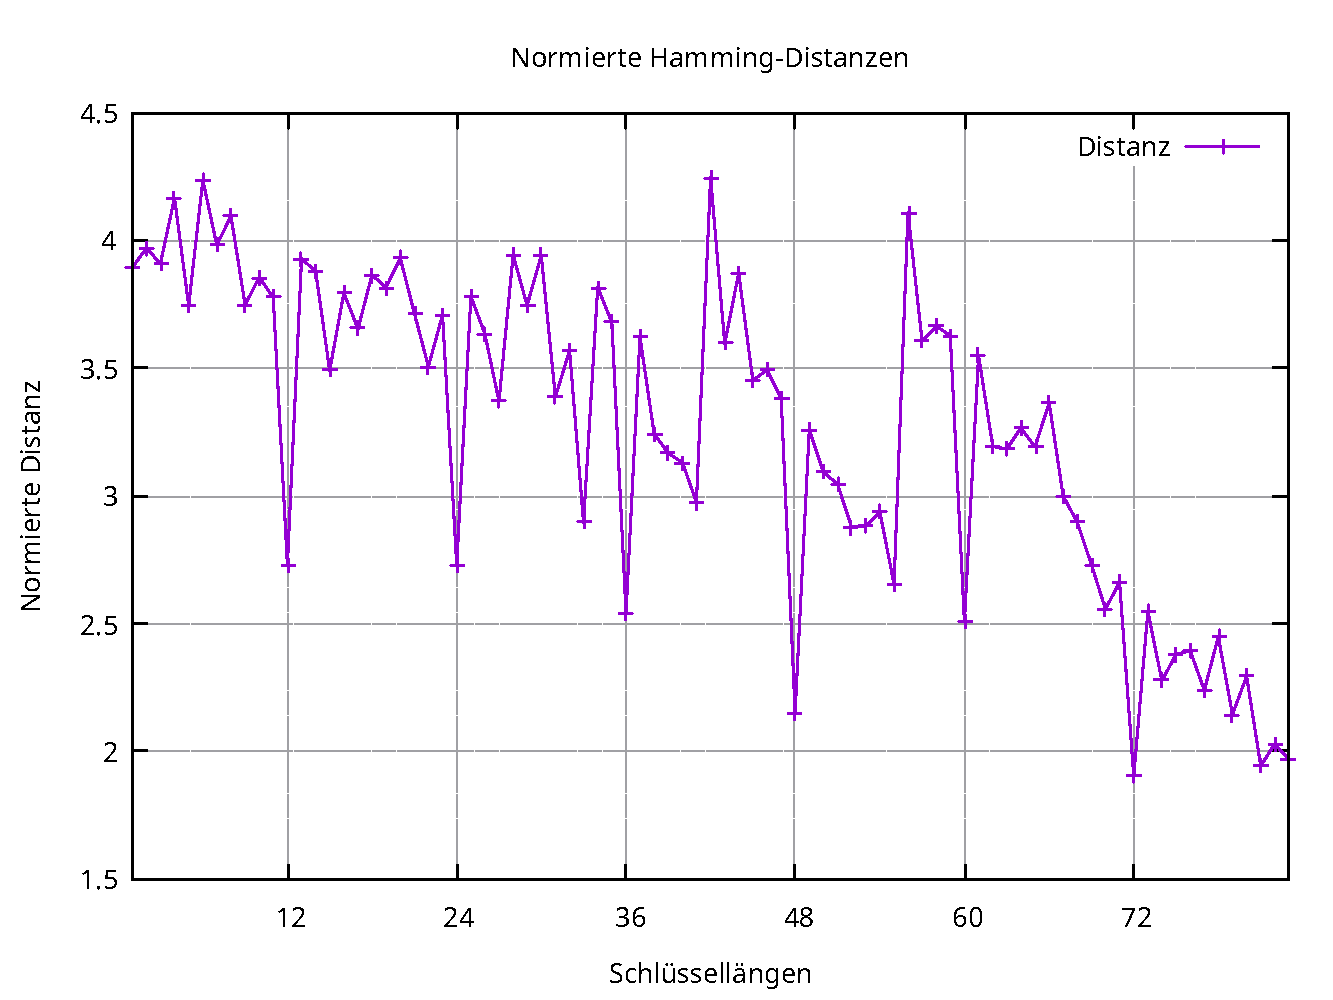
\includegraphics[width=0.8\textwidth]{img/plots/norm_hd_key_12.pdf}
    \caption{Normierte Hamming-Distanzen bei einer Schlüssellänge von 12 und einem 
    168 Zeichen langem Plaintext.}
    \label{fig:avg_hamming_distances}
\end{figure}
Je größer die geschätzte Schlüssellänge ist, desto niedriger wird die normierte 
Hamming-Distanz. Das liegt daran, dass mit einer zunehmenden Blockgrößer der
Durchschnitt der Hamming-Distanz an Aussagekraft verliert. Man kann aber deutliche
Minima bei $12$ und den Vielfachen erkennen. Dementsprechend würde man das erste
dieser Minima als Schlüssellänge verwenden.\newpage
    \section{Aufgabe 18}

\textit{Fortsetzung Aufgabe 11.): Führen sie eine Known Plaintext Attacke gegen den in
Aufgabe 11.) implementierten Cipher durch und ermitteln sie aus den erzeugten
Daten automatisch den für z verwendeten Wert}
\vspace*{1em}\newline
Im Gegensatz zur vorherigen Aufgabe steht ein fester, bekannter Klartext zur Verfügung, welcher in einer „Black-Box“ verschlüsselt wird. Die Verschlüsselung erfolgt intern mit einem zufällig gewählten Schlüssel.
\begin{verbatim}
let plain = "World";
let cipher = black_box(plain);
\end{verbatim}
Die Funktion \texttt{black\_box} nimmt einen Klartext entgegen, generiert intern einen zufälligen Schlüssel im Bereich $[0, 25]$ und verschlüsselt den Text mit der Caesar-Chiffre:
\begin{verbatim}
fn black_box(plain: &str) -> String {
    let key = rng().random_range(0..26);
    caesar_cipher(plain, key) // Implementierung aus Aufgabe 11
}
\end{verbatim}
Ein Beispielversuch mit dieser Methode ergibt folgendes Klartext-Ciphertext-Paar:
\begin{verbatim}
Secret Key:     9
Plain:          World
Cipher:         Fxaum
\end{verbatim}
Da es sich bei der Caesar-Verschlüsselung um eine monoalphabetische Substitution mit fester Verschiebung handelt, genügt es, die Differenz eines Buchstabenpaares (aus Plain- und Ciphertext) zu berechnen, um den verwendeten Schlüssel zu ermitteln.
Seien $P$ der numerische Wert eines Buchstabens aus dem Klartext und $C$ der entsprechende Wert im Geheimtext. Der Schlüssel $S$ ergibt sich dann durch:
\[
S = (C - P) \bmod 26
\]
In der Praxis kann diese Berechnung beispielsweise durch Vergleich des ersten Buchstabenpaares durchgeführt werden:
\begin{verbatim}
let c1 = plain.chars().nth(0).unwrap() as i8;
let c2 = cipher.chars().nth(0).unwrap() as i8;
let key = (c2 - c1).rem_euclid(26);
\end{verbatim}
Wendet man dieses Verfahren auf das obige Beispiel an, so ergibt sich:
\begin{verbatim}
Secret Key:     9
Plain:          World
Cipher:         Fxaum
Calculated Key: 9
\end{verbatim}

\subsection*{Fazit}
Ein Known-Plaintext-Angriff auf eine Caesar-Verschlüsselung lässt sich mit minimalem Aufwand erfolgreich durchführen. 
Bereits ein einziges Zeichenpaar reicht aus, um den verwendeten Schlüssel eindeutig zu rekonstruieren.\newpage
    \section{Aufgabe 19}
\textit{Leiten Sie die kombinatorischen Werte des Geburtstags-Paradoxons her.}
\paragraph{1. } Wie viele Menschen müssen in einem Raum sein, damit die Wahrscheinlichkeit
größer $\nicefrac{1}{2}$, dass eine oder mehr Personen an einem vorgegebene
Tag Geburtstags haben?\vspace*{1em}\newline
Sei $k$ die Anzahl der Personen in einem Raum. Wir betrachten das Gegenereignis, dass von den $k$
Menschen keiner an dem vorgegebenen Tag Geburtstag hat. Das heißt an einem der anderen 364 Tage.
\begin{gather*}    
    \text{\# günstige Fälle} = 364^k\\
    \text{\# mögliche Fälle} = 365^k
\end{gather*}
Sei $X$ eine Zufallszahl, die beschreibt wie viele von $k$ möglichen Menschen an einem vorgegebenen
Tag Geburtstags haben.
\begin{align*}    
    P(X\ge 1) &= 1 - P(X=0) = 1 - \left(\frac{364}{365}\right)^k\\
    0.5 &= 1 - \left(\frac{364}{365}\right)^k\\
    \ln0.5 &= \ln\left(\frac{364}{365}\right)^k= k\cdot \ln\left(\frac{364}{365}\right)\\
    k &= \frac{\ln 0.5}{\ln \frac{364}{365}} = 252.652
\end{align*}
Also ab 253 Personen wäre die Wahrscheinlichkeit, dass zumindest eine Person an einem
vorgegebenen Tag Geburtstag hat größer \nicefrac{1}{2}.
\paragraph{2. } Wie viele Menschen müssen in einem Raum sein,
damit die Wahrscheinlichkeit größer \nicefrac{1}{2} ist, dass zwei
Personen am gleichen Tag Geburtstag haben?\vspace*{1em}\newline
Wir betrachten das Gegenereignis, dass keine zwei der $k$ Personen am gleichen Tag 
Geburtstag haben. Die Anzahl der günstigen Fälle ergibt sich wie folgt:
\[
    \text{\# günstige Fälle} = 365\cdot 364\cdot 363\cdots (365 - k + 1) = \prod_{i = 0}^{k - 1} (365 - i).
\]
Die Gesamtanzahl der möglichen Kombination ist
\[
    \text{\# mögliche Fälle} = 365^k.
\]
Dadurch erhalten wir die Wahrscheinlichkeit, dass alle Personen an unterschiedlichen Tagen
Geburtstag haben.
\[
    P(\text{alle unterschiedlich}) = \frac{\prod_{i = 0}^{k - 1} (365 - i)}{365^k} = \prod_{i = 0}^{k - 1} \frac{365 - i}{365}
\]
Die gesuchte Wahrscheinlichkeit, dass bei $k$ Personen zwei oder mehr am gleichen Tag haben ist dann
\[
    P(\text{zwei oder mehr gleiche}) = 1 - P(\text{alle unterschiedlich}).
\]
Durch numerische Auswertung für verschiedene $k$ erhält man ein Ergebnis $> 0.5$ bei $k = 23$.\newpage
    \section{Aufgabe 20}
\textit{An welcher Stelle des Protokollangriffs gegen digitale Empfangsbestätigungen
ist tatsächlich die Bedingung }
\[
    V_x = E_x\qquad S_x = D_x
\]
\textit{für den Erfolg notwendig? Warum funktioniert das ohne diese Bedingung nicht?}
\vspace*{1em}\newline
Nachdem Mallory die Nachricht von Alice abgefangen hat besitzt er $E_B(S_A(m))$.
Wenn Mallory nun die Nachricht an Bob schickt und vorgibt der Urheber zu sein,
entschlüsselt und überprüft Bob die Nachricht. Er erstellt
\[
    V_M(D_B(E_B(S_A(m))))
\]
An dieser Stelle "`entfernt"' Bob sich aus der Gleichung, da sich $D_B(E_B(\dots))$
aufheben. Es bleibt $V_M(S_A(m))$. Wird nun der gleiche Algorithmus zur Signatur/Verifikation
und zur Ver- und Entschlüsselung verwendet gilt $V_M = E_M$. 
Somit hätte Bob eigentlich $E_M(S_A(m))$. Anschließend schickt Bob die 
signierte Empfangsbestätigung an Mallory.
\[
    V_M(S_B(E_M(S_A(m)))) = E_M(S_B(E_M(S_A(m))))
\]
Mallory kann ohne Schwierigkeiten $E_M(\dots)$ durch $D_M(E_M(\dots))$ entfernen.
Es bleibt 
\[
    S_B(E_M(S_A(m)))
.\]
Aufgrund der Bedingung $S_x = D_x$ ist eine Signatur gleich einer Entschlüsselung mit
dem Privaten Schlüssel.
\[
    S_B(E_M(S_A(m))) = D_B(E_M(D_A(m)))
\]
Mallory kann nun wie in der VO beschrieben zuerst den Public Key von Bob zur Verschlüsselung,
dann seinen Private Key zur Entschlüsselung und zuletzt den Public Key von Alice verwenden, um
die Nachricht $m$ zu erhalten.
\newpage
    \section{Zeitaufwand}
Zeiteinheiten sind in Stunden [h].
\begin{table}[h]
    \begin{tabular}{l|ccc|r}
        Aufgabe & Coding & Recherche & Schreiben & $\sum$\\\hline
        Aufgabe 14 & 0 & 0.5 & 1 & 1.5 \\
        Aufgabe 15 & 5 & 0.5 & 6 & 11.5 \\
        Aufgabe 16 & 1.5 & 1.5 & 2 & 5 \\\hline
        $\sum$     & 6.5 & 2.5   & 9 & 18
    \end{tabular}
\end{table}

\end{document}